\section{Vergleich der implementierten Lösungsverfahren} \label{sec:BenchmarkErgebnisse_MetaheuristischeVerfahren}

Die implementierten Lösungsverfahren wurden über die vollständigen Instanzsets m1, m2, n0, n1 und j20 miteinander verglichen. Tabelle \ref{tab:evaluation_solver_n1} zeigt die quantitativen Ergebnisse für das Instanzset n1 auf, während im Anhang \ref{sec:WeitereAuswertung_Metaheuristiken} die Ergebnisse der weiteren Instanzsets entnommen werden können. 
% Für den Mittelwertvergleich der abweichenden Makespans zu den Optima und für den Mittelwertvergleich der Robustheitswerte der optimalen Zeitplänen wurden Signifikanztests vollzogen. Als Signifikanztest wurde der Kruskal-Wallis-Test selektiert. Dieser Test ist für mehrere ($> 2$) unabhängige, nicht normalverteilte Gruppierungen vorgesehen. Die fünf Lösungsverfahren mit den je vier durchlaufenden Iterationen folgen keiner Normalverteilung und stellen voneinander unabhängige Gruppen dar. Das Signifikanzniveau zur Ablehnung oder Annahme der Nullhypothese $H_0$ wird auf $\alpha = 0.05$ festgelegt. 

\begin{table}[H]
\centering
\resizebox{0.91\textwidth}{!}\\
Solver & Iteration &          &  &  & \\
\midrule
RandomSolver & 500  &     6.17 & 3.47 &      14.99 & 4.11 &   100.00 &    7.69 \\
                 & 1000 &     5.30 & 3.15 &      15.21 & 5.06 &   100.00 &   10.52 \\
                 & 2500 &     4.40 & 2.76 &      15.55 & 5.34 &   100.00 &   14.91 \\
                 & 5000 &     3.76 & 2.57 &      15.66 & 5.14 &   100.00 &   19.47 \\ \hline
HillClimbing & 500  &     2.61 & 2.97 &      17.96 & 6.02 &   100.00 &   54.63 \\
                 & 1000 &     2.48 & 2.88 &      17.88 & 6.01 &   100.00 &   56.67 \\
                 & 2500 &     2.42 & 2.87 &      17.96 & 5.99 &   100.00 &   55.26 \\
                 & 5000 &     2.41 & 2.78 &      17.73 & 6.05 &   100.00 &   56.67 \\ \hline
TabuSearch & 500  &     1.85 & 2.37 &      18.00 & 6.44 &   100.00 &   64.84 \\
                 & 1000 &     1.37 & 2.00 &      17.75 & 6.64 &   100.00 &   75.35 \\
                 & 2500 &     0.94 & 1.66 &      17.54 & 6.64 &   100.00 &   83.05 \\
                 & 5000 &     0.72 & 1.43 &      17.48 & 6.69 &   100.00 &   87.76 \\ \hline
SimulatedAnnealing & 500  &     2.60 & 2.69 &      17.81 & 6.38 &   100.00 &   50.39 \\
                 & 1000 &     1.65 & 2.05 &      17.81 & 6.56 &   100.00 &   63.42 \\
                 & 2500 &     0.95 & 1.46 &      17.40 & 6.88 &   100.00 &   78.96 \\
                 & 5000 &     0.59 & 1.00 &      17.29 & 6.96 &   100.00 &   87.91 \\ \hline
GeneticAlgorithm & 500  &     2.23 & 2.35 &      17.62 & 6.47 &   100.00 &   48.04 \\
                 & 1000 &     1.03 & 1.39 &      17.09 & 6.69 &   100.00 &   73.63 \\
                 & 2500 &     0.49 & 0.88 &      17.21 & 6.72 &   100.00 &   87.13 \\
                 & 5000 &     0.39 & 0.76 &      17.30 & 6.62 &   100.00 &   91.21 \\
\bottomrule
\end{tabular}
}
\caption{Vergleich der Lösungsverfahren für das Instanzset n1}
\source{Eigene Darstellung}
\label{tab:evaluation_solver_n1}
\end{table}

Beim direkten Vergleich der Lösungsverfahren lässt sich erkennen, dass das zu-fällige Generieren von Zeitplänen die schlechteste der implementierten Varianten darstellt. Für das Instanzset n1 konnten z. B. nur 19,47 \% optimale Lösungen gefunden werden. Dieses Lösungsverfahren eignet sich jedoch für das m1-Instanzset außerordentlich gut, welches mit einer niedrigen Aktivitäts- und Modusanzahl das einfachste Instanzset der Evaluation darstellt und somit auch die geringste Anzahl an Permutationen aufweist. Hierbei konnten die besten Ergebnisse in Bezug auf die gemittelte Abweichung der Makespans, der Robustheit und der Optimum-Rate erreicht werden. Hill Climbing stellt eine Verbesserung zur zufälligen Generierung von Lösungen dar. Dennoch eignet sich das Verfahren im Vergleich auf die implementierten Metaheuristiken weniger, da sowohl die Abweichung zu den besten Makespans als auch die Rate der optimalen Lösungen am geringsten ist. Eine mögliche Begründung liegt darin, dass beim Erreichen von lokalen Optima diese nicht mehr verlassen werden können. Der integrierte Tabu Suche-Algorithmus erreicht schon mit einer geringen Anzahl an Iterationen ($i = 500$) bereits gute Ergebnisse und stellt auch mit höheren Iterationen für sowohl einfachere als auch komplexe Instanzsets solide Ergebnisse. Simulated Annealing liefert über alle Instanzsets hinweg ähnliche Ergebnisse zur Tabu Suche, jedoch mit höheren Abweichungen. Der umgesetzte genetische Algorithmus liefert ab $i = 1 000$ Iterationen in den meisten Instanzsets die besten Ergebnisse in Bezug auf die Makespanabweichung und der Optimumsrate. Abbildung \ref{fig:evaluation_solver_n1_makespan_boxplot} und \ref{fig:evaluation_solver_n1_robust_boxplot} stellen Boxplots dar, welche die weiteren deskriptiven Statistiken der einzelnen Lösungsvarianten grafisch aufführen. 

\begin{figure}[H]

    \begin{subfigure}{0.497\linewidth}
        \centering
        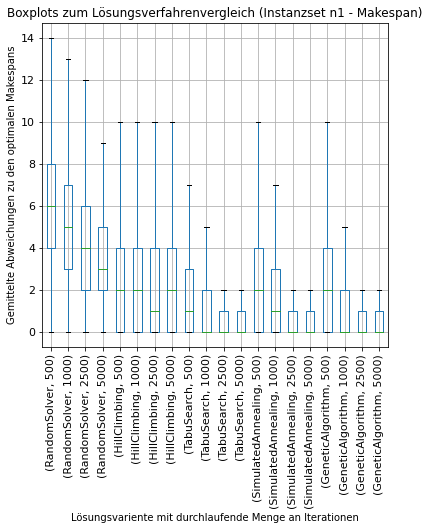
\includegraphics[width=\linewidth]{assets/img/05_Evaluation/Boxplot_n1_Makespan.png}
        \caption{Makespanabweichungen von $C_{max}$}
        \label{fig:evaluation_solver_n1_makespan_boxplot}
    \end{subfigure}
    \hfill
    \begin{subfigure}{0.497\linewidth}
        \centering
        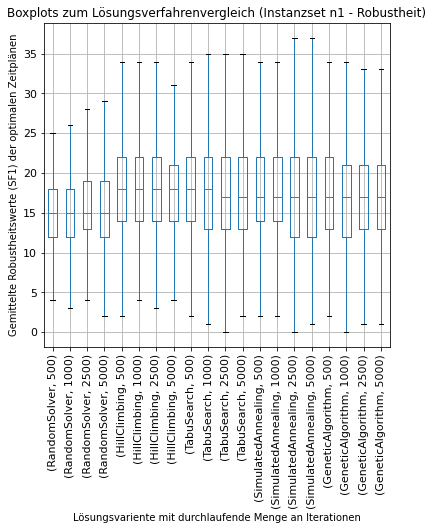
\includegraphics[width=\linewidth]{assets/img/05_Evaluation/Boxplot_n1_Robust.png}
        \caption{Robustheit $\Omega^{SF1}$}
        \label{fig:evaluation_solver_n1_robust_boxplot}
    \end{subfigure}
    
    \caption{Boxplot der implementierten Lösungsverfahren für das Instanzset m1 in Bezug auf die gemittelte a) und b)}
    \source{Eigene Darstellungen}
\end{figure}
